\chapter{Metodologia}

Nesta seção, descrevemos a metodologia adotada para desenvolver e testar o algoritmo de avaliação automática de respostas dissertativas. O processo abrange desde a formatação dos dados até a comparação dos resultados gerados pelo algoritmo com as avaliações realizadas pelos docentes. De forma visual o processo geral pode ser visto na Figura \ref{figure:29}

\begin{figure}[h!]
\centering
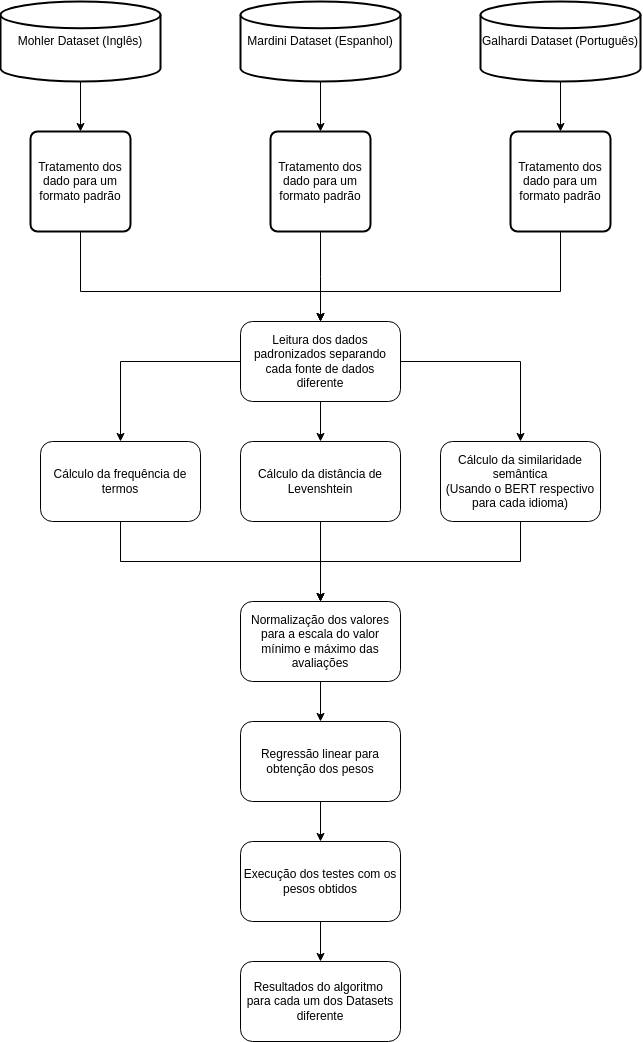
\includegraphics[width=0.8\textwidth]{img/tccFlux.png}
\caption{Diagrama do fluxo completo do algoritmo}\label{figure:29}
\end{figure}

\FloatBarrier

Na metodologia, de forma geral, foram retirados dos textos disponíveis nas bases de dados os três fatores que são usados regressão linear e posteriormente nos testes de geração de avaliações. Esses fatores são:

\begin{itemize} 
  \item \textbf{As propriedades léxicas do texto:} O primeiro fator será levado em consideração fazendo uso das frequências de termos de cada texto. 
  \item \textbf{As propriedades da sintaxe do texto:} O segundo fator será levado em consideração fazendo uso da distância de Levenshtein. 
  \item \textbf{As propriedades da semântica do texto:} O terceiro fator será levado em consideração fazendo uso dos valores de similaridade semântica fornecidos pelos embeddings gerados pelo modelo BERT. 
\end{itemize}

A métrica utilizada na metodologia pode ser matemáticamente descrita como o exemplo da Equação 1, que contém a equação de uma média ponderada.
\begin{equation}
Métrica = \frac{fator1 \times peso_{1} + fator2 \times peso_{2} + fator3 \times peso_{3}}{\sum_{i=1}^{3}peso_{i}}
\label{eq:1}
\end{equation}

\section{Pipeline de execução do algoritmo}

O pipeline de execução do algoritmo compreende várias etapas, desde a preparação dos dados até a análise dos resultados. As etapas podem ser detalhadas da seguinte forma:

\subsection{Formatação dos Dados}

A primeira etapa envolve a formatação dos dados oriundos de diferentes bases, convertendo-os em um modelo comum. 

Uma das principais dificuldades encontradas inicialmente no presente trabalho foi o tratamento de dados provenientes de múltiplas bases em diferentes idiomas, cada uma com formatos e estruturas distintas. 

Isso exigiu a implementação de algoritmos de pré-processamento e normalização de texto para garantir a consistência dos dados antes da análise. Isso foi fundamental para desenvolver abordagens eficazes de tratamento de dados em inglês, espanhol e português.

Isso garante a padronização dos dados, facilitando o processamento subsequente. A estrutura de dados é definida como demonstrado no diagrama da Figura \ref{figure:28}, onde cada entrada é tipada e preparada para a análise, no fim essas informações são salvas em arquivo no formato \textit{.json} para facilitar a leitura com auxílio de bibliotecas prontas na linguagem de programação \textit{Python}.

\begin{figure}[h!]
\centering
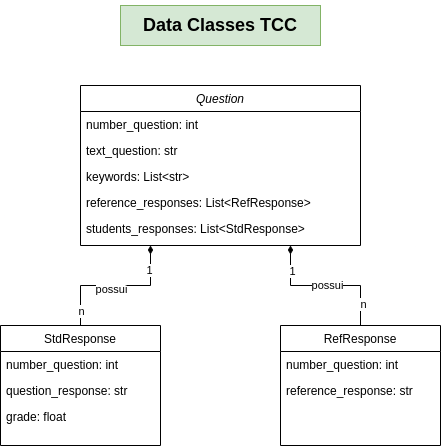
\includegraphics[width=0.6\textwidth]{img/DataClassModelsTCC.png}
\caption{Modelo de padronização dos dados representados como classes}\label{figure:28}
\end{figure}

\FloatBarrier

\subsection{Extração e Normalização dos Fatores}

Após a formatação, os dados são processados pelo algoritmo para a extração de três fatores principais que influenciam a avaliação. Primeiramente, é feito o cálculo da distância de Levenshtein entre o texto da resposta de referência do professor e a resposta de um aluno disponível na base de dados, retornando um valor para avaliar a proximidade da sintaxe dos dois textos. Em seguida, o cálculo da frequência de termos usando \textit{Count Vectorization} é feito para ambos os textos, e a comparação entre os vetores gerados para eles é feita usando a distância de cosseno, gerando um valor para avaliar a semelhança léxica dos textos.

Depois disso, utilizando o modelo BERT, os embeddings dos textos são calculados. O BERT utiliza uma técnica chamada "WordPiece tokenization" para dividir o texto em pedaços menores, chamados de "tokens". Cada token é então convertido em um vetor de números reais através de uma camada de embeddings. Esses embeddings capturam o contexto e o significado das palavras no texto. Posteriormente, os embeddings de cada texto são organizados em matrizes e manipulados para calcular a similaridade entre eles utilizando a distância de cosseno, o que resulta em um valor que representa a similaridade semântica entre os dois textos.

Esse processo é repetido algumas vezes apenas para o fator semântico, pois existem modelos diferentes do BERT em cada idioma e versões diferentes (\textit{Base} e \textit{Large}). É necessário utilizar os dados gerados por cada um dos modelos para avaliar o desempenho do algoritmo com cada um deles.

No fim, todos os fatores são normalizados com base nos valores mínimos e máximos das notas fornecidas pelos professores. A normalização é crucial para garantir que os fatores se situem dentro da mesma escala na qual as notas devem ser avaliadas.

\subsection{Regressão Linear}

Com os fatores normalizados, a próxima etapa é a aplicação de uma regressão linear. A regressão é treinada comparando os fatores extraídos com as notas das avaliações dos professores. Isso permite determinar os pesos específicos para cada fator. Os pesos obtidos são essenciais para a fase subsequente, onde serão usados para gerar novas avaliações. Além dos pesos, com a regressão também é possível obter os valores do EQM (\textit{Mean Squared Error} ou MSE) e do EMA (\textit{ Mean Absolute Error} ou MAE).

\subsection{Geração de Avaliações}

Utilizando os pesos determinados pela regressão linear, o algoritmo gera avaliações automáticas para um conjunto de dados separados. Esses dados são as respotas dos alunos em comparadas com as referências dos professsores, porém nesse momento os três fatores são retirados dos textos e logo em seguida uma avaliação de nota é gerando fazendo o cálculo da média ponderada, para isso são usados, em conjunto com os valores de cada fator, os valores de cada peso que foram determinados anteriormente na regressão linear. Após isso, ainda nesta etapa, os valores das avaliações geradas pelo algoritmo são guardados para serem comparados com as avaliações feitas pelos próprios professores para as mesmas respotas de alunos disponíveis nas bases de dados, assim podermos constatar se há semelhança entre os valores de ambas as avaliações, do algoritmo e dos professores.

\subsection{Comparação e Cálculo de Acurácia}

Finalmente, as avaliações geradas pelo algoritmo são comparadas com as notas originais fornecidas pelos professores na base de dados. Essas comparações são feitas dividindo o conjunto de dados em diferentes quantias de valores. Primeiramente, 60\% dos dados são usados para o treino da regressão na etapa anterior e 40\% dos dados são usados para testes na etapa atual. Em seguida, os valores de treino e testes são ajustados para 70\% e 30\%, respectivamente. Essa alteração é feita sucessivamente para os valores de 80\% e 20\% até os valores finais de 90\% e 10\%. Esse ciclo é repetido para todas as bases de dados e todas as versões dos modelos \textit{BERT}. A precisão dessas avaliações é verificada em termos de acurácia percentual. A acurácia média é então calculada para todas as avaliações geradas nos testes, permitindo avaliar o desempenho do algoritmo.

\subsection{Execução do algoritmo em diferentes bases e modelos}

Todo o ciclo de metodologia é executado múltiplas vezes para cada uma das bases de dados e das diferentes versões dos modelos, afim de obter a maior quantidade de dados possíveis para avaliação da acurácia do algoritmo no final em vários casos e observar em quais casos os resultados obtidos foram melhores.

\subsection{Otimização do algoritmo}

No decorres do desenvolvimento do presente trabalho, uma dificuldade enfrentada foi otimizar a execução do algoritmo para lidar com grandes volumes de dados de forma eficiente. Isso exigiu a implementação de estratégias avançadas de otimização, como a paralelização com \textit{multi-threading}, a programação dinâmica, uso de protocolos como \textit{Open MPI} e a execução dos modelos na \textit{GPU} com \textit{CUDA}.

A paralelização com \textit{multi-threading} permitiu que o algoritmo executasse múltiplas tarefas em paralelo, acelerando o processamento de grandes conjuntos de dados. A programação dinâmica otimizou o uso de recursos computacionais e reduziu a complexidade algorítmica, garantindo uma execução mais eficiente do algoritmo e menos repetições desnecessárias de trechos de código. A divisão de processos com protocolo \textit{MPI} permitiu que diferentes partes do algoritmo trocassem dados de forma assíncrona e coordenada, dividindo a carga de trabalho. Já a execução dos modelos na \textit{GPU} com \textit{CUDA} acelerou o processamento de dados, aproveitando o poder de processamento das \textit{GPU's} para lidar com grandes volumes de dados de forma eficiente.

Essas técnicas de otimização garantiram uma execução eficiente do algoritmo, permitindo lidar com grandes volumes de dados e garantir tempos de execução adequados. Antes desse processo de otimização, o tempo estimado de execução do algoritmo estava em cerca de 10 dias cada vez que era rodado. Após as otimizações do código, o algoritmo pode ser executado completamente em cerca de 40 minutos. A experiência técnica e o conhecimento especializado obtidos ao longo da graduação foram fundamentais para superar os desafios enfrentados durante o desenvolvimento do algoritmo e garantir sua eficácia e otimização nos tempos de execução.

\section{\textit{Datasets utilizados}}

Para este projeto de avaliação automática de respostas curtas, foram utilizadas três bases de dados distintas, cada uma em um idioma específico. A primeira base de dados consiste em um conjunto de questões de Biologia em português, a segunda base de dados é composta por questões de Literatura em espanhol e a terceira base de dados contém questões de Ciência da Computação em inglês.

A base de dados em português foi apresentada por \textcite{datasetPort} criada em 2020, contendo cerca de 15 questões e 23350 respostas de alunos.

Além disso, o conjunto de dados em espanhol apresentado por \textcite{datasetEsp} em 2023, contem cerca de 20 questões e 3770 respostas de alunos.

Por fim, a base de dados em inglês empregada foi apresentada por \textcite{datasetEng} em 2009, contando com 85 questões e 3645 respostas de alunos.

% \begin{figure}[h!]
% 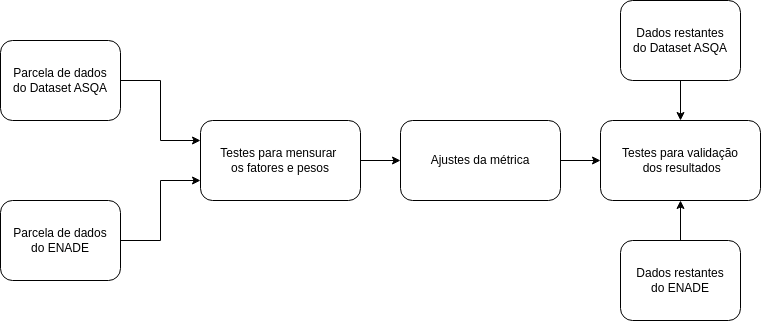
\includegraphics[width=\textwidth]{img/diagramasTcc.png}
% \caption{Diagrama geral das etapas do processo.}\label{figure:4}
% \end{figure}

% olhar depois:

% https://www.researchgate.net/publication/337412528_Avaliacao_Automatica_de_respostas_discursivas_curtas_baseado_em_tres_dimensoes_linguisticas

% https://revistas.unoeste.br/index.php/ce/article/view/4595

% https://physionet.org/content/radqa/1.0.0/

% https://ppgee.propesp.ufpa.br/ARQUIVOS/teses/tese_abntex_final.pdf

% dataset search google

\newpage